\documentclass[svgnames,11pt]{beamer}
\setbeamercolor{structure}{fg=SlateGray}
\usetheme{Goettingen}
\input{/home/tof/Documents/Cozy/latex-include/preambule_commun.tex}
%\usepackage{pgfpages}
%\setbeameroption{show notes on second screen=left}
\author[]{Christophe Viroulaud}
\title{Pokémon Go}
\date{}
%\logo{}
%\institute{Seconde SNT}
\institute{Première NSI}
%\institute{Terminale NSI}
\setbeamertemplate{navigation symbols}{}
\setbeamertemplate{footline}[frame number]

\begin{document}
\begin{frame}
    \titlepage
    \note{\fcolorbox{black}{red}{pokemon.zip sur site (pokedex.csv+dossier photos)}}
\end{frame}

\section{Problématique}
\begin{frame}
    \frametitle{Problématique}

    Le jeu pour smartphone \emph{Pokemon Go} reprend l'univers du manga éponyme. Il utilise la réalité augmentée pour donner une expérience utilisateur nouvelle.
    \begin{center}
        \centering
        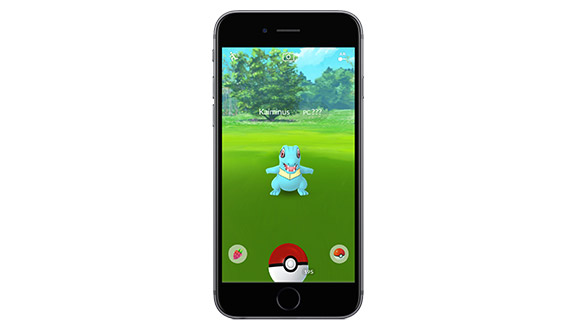
\includegraphics[width=7cm]{ressources/pokemongo.jpg}
        \captionof{figure}{Illustration du jeu Pokémon GO}
    \end{center}


\end{frame}

\begin{frame}
    \frametitle{}

    Devant le succès du jeu des communautés se créent et tentent d'établir des stratégies pour optimiser leurs résultats.

    \begin{center}
        {\Large On se propose de construire un programme pour aider les joueurs dans leurs quêtes.}
    \end{center}
\end{frame}
\section{Informations disponibles}
\begin{frame}
    \frametitle{Informations disponibles}

    Quand on joue à \emph{Pokémon Go} on trouve des Pokémon sur notre chemin, mais également des œufs. Il faut parcourir une certaine distance pour faire éclore un œuf. Enfin, il est possible de faire évoluer un Pokémon à l'aide de friandises.

    Un fichier de données (\emph{pokedex.csv}) recense l'ensemble des Pokémons utilisables dans le jeu.

\end{frame}

\begin{frame}
    \frametitle{Attributs du fichier}

    \begin{itemize}
        \item num: Number of the Pokémon in the official Pokédex
        \item name: Pokémon name
        \item img: URL to an image of this Pokémon
        \item type: Pokémon type
        \item height: Pokémon height (m)
        \item weight: Pokémon weight (kg)
        \item candy: type of candy used to evolve Pokémon or given when transfered
        \item candy\_count: amount of candies required to evolve
        \item egg: Number of kilometers to travel to hatch the egg
        \item weakness: Types of Pokémon this Pokémon is weak to
        \item next\_evolution: Number of evolution of Pokémon
    \end{itemize}

\end{frame}

\begin{frame}
    \frametitle{}

    \begin{activite}
        \begin{enumerate}
            \item Ouvrir le fichier \emph{pokedex.csv} pour observer les données fournies.
            \item Créer un programme \emph{pokemon.py}.
            \item Importer les données du pokedex dans un tableau de dictionnaires \textbf{\texttt{pokedex}}. Typer correctement les données de poids et de taille.
        \end{enumerate}
    \end{activite}

\end{frame}
\begin{frame}[fragile]
    \frametitle{Correction}

    \begin{center}
        \begin{lstlisting}[language=Python,basicstyle=\small]
fichier = open("pokedex.csv")
data = csv.DictReader(fichier)
pokedex = []
for pokemon in data:
    dico = {}
    for cle, val in pokemon.items():
        # validation des données
        if cle == "height" or cle == "weight":
            val = float(val)

        dico[cle] = val
    # ajout du pokemon dans le tableau
    pokedex.append(dico)
fichier.close()
\end{lstlisting}
        \captionof{code}{Importation des données}
        \label{CODE}
    \end{center}

\end{frame}

\section{Interface graphique}

\begin{frame}
    \frametitle{Interface graphique}

    L'interface permet à l'utilisateur d'interagir avec les données à l'aide de boutons, boîtes de dialogue\dots
    \begin{center}
        \centering
        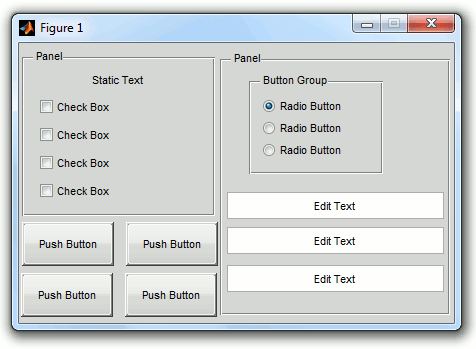
\includegraphics[width=7cm]{ressources/interface.png}
        \captionof{figure}{Exemple d'interface graphique}
        \label{IMG}
    \end{center}

\end{frame}
\subsection{Bibliothèque tkinter}
\begin{frame}[fragile]
    \frametitle{Bibliothèque tkinter}

    La bibliothèque tkinter fournit des \emph{composants (widgets)} pour construire une interface graphique simple.
    \begin{center}
        \begin{lstlisting}[language=Python,basicstyle=\small,xrightmargin=1em]
import tkinter
from tkinter import ttk

#création de la fenêtre
fenetre = tkinter.Tk()
fenetre.title("Pokemon Go")

# la construction des composants se placera ici

# dernière ligne du programme: met à jour les variables 
fenetre.mainloop()
\end{lstlisting}
        \captionof{code}{Créer une fenêtre d'interface}
        \label{interface}
    \end{center}

\end{frame}

\subsection{Ajouter un composant}
\begin{frame}
    \frametitle{Ajouter un composant}

    L'ajout d'un composant se déroule en trois étapes:
    \begin{itemize}
        \item Créer le composant.
        \item Placer le composant dans l'interface.
        \item Remplir le composant.
    \end{itemize}

\end{frame}
\begin{frame}[fragile]
    \frametitle{Exemple}

    \begin{center}
        \begin{lstlisting}[language=Python,basicstyle=\small]
# création
etiquette = tkinter.Label(fenetre)
# placement
etiquette.pack()
# remplissage
etiquette["text"] = "Bonjour"
\end{lstlisting}
        \captionof{code}{Placer un \emph{label}} dans la fenêtre
        \label{label}
    \end{center}

\end{frame}
\begin{frame}
    \frametitle{}
    \begin{activite}
        Construire une interface avec trois labels \textbf{\texttt{nom, poids, taille}}.
    \end{activite}


\end{frame}

\begin{frame}[fragile]
    \frametitle{Correction}
    \begin{center}
        \begin{lstlisting}[language=Python,basicstyle=\small]
label_nom = tkinter.Label(fenetre)
label_nom.pack()
label_nom["text"] = "Bulbasaur"

label_poids = tkinter.Label(fenetre)
label_poids.pack()
label_poids["text"] = "6.9kg"

label_taille = tkinter.Label(fenetre)
label_taille.pack()
label_taille["text"] = "0.71m"
\end{lstlisting}
        \captionof{code}{Création d'une carte Pokémon}
        \label{CODE}
    \end{center}



\end{frame}
\begin{frame}
    \frametitle{Correction}

    \begin{center}
        \centering
        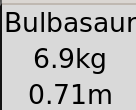
\includegraphics[width=3cm]{ressources/carte0.png}
        \captionof{figure}{Interface obtenue}
        \label{IMG}
    \end{center}

\end{frame}
\begin{frame}[fragile]
    \frametitle{Placement plus précis}
    La méthode \textbf{\texttt{pack}} place les éléments les uns en dessous des autres. Il existe la méthode \textbf{\texttt{grid}} qui utilise un système de coordonnées.
    \begin{center}
        \begin{lstlisting}[language=Python]
etiquette.grid(column=0, row=0)
\end{lstlisting}
        \captionof{code}{Place le composant \textbf{\texttt{etiquette}}} aux coordonnées (0,0)
        \label{CODE}
    \end{center}
    \begin{aretenir}[Commentaire]
        On ne peut pas utiliser deux géométries de placement différents (\textbf{pack, grid}) dans un même bloc.

    \end{aretenir}


\end{frame}
\begin{frame}
    \frametitle{}
    \begin{activite}
        Présenter les trois labels sous la forme d'une grille.
        \begin{center}
            \begin{tabular}{cc}
                nom   &        \\
                poids & taille \\
            \end{tabular}
        \end{center}
    \end{activite}


\end{frame}

\begin{frame}[fragile]
    \frametitle{Correction}

    \begin{center}
        \begin{lstlisting}[language=Python, basicstyle=\small]
label_nom = tkinter.Label(fenetre)
label_nom.grid(column=0, row=0)
label_nom["text"] = "Bulbasaur"

label_poids = tkinter.Label(fenetre)
label_poids.grid(column=0, row=1)
label_poids["text"] = "6.9kg"

label_taille = tkinter.Label(fenetre)
label_taille.grid(column=1, row=1)
label_taille["text"] = "0.71m"
\end{lstlisting}
        \captionof{code}{}
        \label{CODE}
    \end{center}

\end{frame}
\subsection{Construire par bloc}
\begin{frame}
    \frametitle{Construire par bloc}

    Pour organiser les composants de manière plus ordonnée, il est préférable de ne pas tous les plaquer directement dans la fenêtre \emph{tkinter} principale. On crée alors des blocs (\textbf{\texttt{Frame}}) pour découper notre interface.


\end{frame}
\begin{frame}[fragile]
    \frametitle{}

    \begin{center}
        \begin{lstlisting}[language=Python, basicstyle=\small]
# création d'un bloc
bloc_carte = tkinter.Frame(fenetre)

# on plaque les composants dans le bloc
label_nom = tkinter.Label(bloc_carte)
label_nom.grid(column=1, row=0)

label_poids = tkinter.Label(bloc_carte)
label_poids.grid(column=0, row=1)

label_taille = tkinter.Label(bloc_carte)
label_taille.grid(column=1, row=1)

# On plaque le bloc dans la fenêtre
bloc_carte.pack()
\end{lstlisting}
        \captionof{code}{Création d'un bloc}
        \label{bloc}
    \end{center}

\end{frame}
\begin{frame}
    \frametitle{}

    \begin{aretenir}[Remarque]
        Dans le code \ref{bloc}, la \emph{Frame} \textbf{\texttt{bloc\_carte}} a utilisé une géométrie \textbf{\texttt{grid}} alors que la fenêtre principale c'est \textbf{\texttt{pack}} qui est utilisé. Il n'y a pas d'incompatibilités car il s'agit de deux blocs différents.
    \end{aretenir}

\end{frame}

\subsection{Remplissage des labels}
\begin{frame}
    \frametitle{Remplissage des labels}

    Pour remplir le texte des composants on peut choisir de créer une fonction.
    \begin{activite}
        Écrire la fonction \textbf{\texttt{remplir\_carte(num\_pok: int) $\rightarrow$ None}} qui remplit les trois labels créés en fonction du numéro de Pokémon choisi dans le Pokédex.
    \end{activite}
\note{Le tableau \textbf{\texttt{pokedex}} est utilisé ici comme une variable globale $\rightarrow$ pour faciliter l'usage du callback plus tard.}
\end{frame}
\begin{frame}[fragile]
    \frametitle{Correction}
    \begin{center}
        \begin{lstlisting}[language=Python, basicstyle=\small]
def remplir_carte(num_pok: int) -> None:
    # choix du pokemon dans le pokedex
    pok = pokedex[num_pok]

    label_nom["text"] = pok["name"]
    label_poids["text"] = str(pok["weight"])+"kg"
    label_taille["text"] = str(pok["height"])+"m"
\end{lstlisting}
        \captionof{code}{Fonction de remplissage}
        \label{CODE}
    \end{center}

    \begin{aretenir}[Commentaire]
        La fonction utilise ici des variables du programme principal. Avec nos connaissances actuelles, c'est la manière la plus simple de procéder.
    \end{aretenir}
\end{frame}
\begin{frame}[fragile]
    \frametitle{Correction}

    Dans le programme principal, l'appel \ref{appel} après la création des labes, affiche les informations du Pokemon 12.

    \begin{center}
        \begin{lstlisting}[language=Python, basicstyle=\small]
remplir_carte(12)
\end{lstlisting}
        \captionof{code}{Remplissage des labels}
        \label{appel}
    \end{center}

\end{frame}

\subsection{Gestion des images}
\begin{frame}[fragile]
    \frametitle{Gestion des images}

    L'affichage d'une image demande un peu plus de travail. Il faut créer un objet \textbf{\texttt{PhotoImage}} qui sera ensuite affiché dans un composant \textbf{\texttt{label\_photo}}. Commençons par créer le composant.
    \begin{center}
        \begin{lstlisting}[language=Python, basicstyle=\small]
label_photo = tkinter.Label(bloc_carte)
label_photo.grid(column=1, row=0)  
\end{lstlisting}
        \captionof{code}{\textbf{\texttt{label\_photo}} est placé à droite de \textbf{\texttt{label\_nom}}}
        \label{CODE}
    \end{center}

\end{frame}

\begin{frame}[fragile]
    \frametitle{}

    Il faut ensuite modifier la fonction \textbf{\texttt{remplir\_carte}} pour afficher la photo.

    \begin{center}
        \begin{lstlisting}[language=Python, basicstyle=\small]
def remplir_carte(num_pok: int) -> None:
    global photo # garde une référence de l'image

    pok = pokedex[num_pok]

    # affichage de l'image
    photo = tkinter.PhotoImage(file=pok["img"])
    label_photo["image"] = photo

    label_nom["text"] = pok["name"]
    label_poids["text"] = str(pok["weight"])+"kg"
    label_taille["text"] = str(pok["height"])+"m"
\end{lstlisting}
    \end{center}
    \begin{aretenir}[Commentaire]
        La ligne 2 évite que le \emph{garbage collector} efface l'image à la sortie de la fonction. Cette notion est hors programme.
    \end{aretenir}
\end{frame}
\section{Interaction entre les composants}
\begin{frame}
    \frametitle{Interaction entre les composants}

    Notre programme n'est pour l'instant que peut utile: il faut changer \emph{en dur (c'est à dire dans le programme)} le numéro du Pokémon à afficher. La prochaine étape consistera à créer une liste de choix dans l'interface graphique pour changer dynamiquement la carte à afficher.


\end{frame}
\subsection{Liste de choix: \textbf{\texttt{Combobox}}}
\begin{frame}
    \frametitle{\textbf{\texttt{Combobox}}}

Pour afficher les noms des Pokémons dans une liste de choix, il faut d'abord construire un tableau contenant tous ces noms.
\begin{activite}
Construire par compréhension le tableau \textbf{\texttt{noms\_affiches}} des noms de tous les Pokémons du Pokédex.
\end{activite}

\end{frame}
\begin{frame}[fragile]
    \frametitle{Correction}

\begin{center}
\begin{lstlisting}[language=Python,basicstyle=\small,xleftmargin=0em,xrightmargin=0em,numbers=none]
noms_affiches = [pokemon["name"] for pokemon in pokedex]
\end{lstlisting}
\captionof{code}{Tableau des noms}
\label{CODE}
\end{center}  

\end{frame}
\begin{frame}[fragile]
    \frametitle{\textbf{\texttt{Combobox}}}

    Le composant \textbf{\texttt{Combobox}} crée une liste de choix.
    \begin{center}
        \begin{lstlisting}[language=Python,basicstyle=\small]
# création du composant
combo_pok = ttk.Combobox(fenetre, values=noms_affiches)
# valeur par défaut
combo_pok.current(0)
# placement
combo_pok.pack()   
\end{lstlisting}
        \captionof{code}{Création du composant}
        \label{CODE}
    \end{center}

\end{frame}
\subsection{Choisir un Pokémon: un événement}
\begin{frame}[fragile]
    \frametitle{Choisir un Pokémon: un événement}

    Notre interface \emph{tkinter} attend en permanence une action de l'utilisateur. Quand ce dernier change le Pokémon sélectionné dans la \textbf{\texttt{Combobox}}, un \emph{événement} se produit. L'interface \emph{écoute} les événements.

    \begin{center}
    \begin{lstlisting}[language=Python,basicstyle=\small,xleftmargin=0.3em,xrightmargin=0.3em]
combo_pok.bind("<<ComboboxSelected>>", callback_combo)
\end{lstlisting}
    \captionof{code}{Écouteur sur la \textbf{\texttt{Combobox}}}
    \label{CODE}
    \end{center}
Il faut maintenant qu'elle sache comment réagir.
\end{frame}
\begin{frame}[fragile]
    \frametitle{Fonction de rappel (\emph{callback})}

Quand l'utilisateur change la sélection dans la liste de choix, la fonction \textbf{\texttt{callback\_combo}} est appelée. C'est une \textbf{fonction de rappel (callback)}. Un unique paramètre (noté ici \textbf{\texttt{event}}) est passé automatiquement à la fonction. Ce paramètre contient des informations sur le choix effectué.
\begin{center}
\begin{lstlisting}[language=Python,basicstyle=\small]
def callback_combo(event):
    # num contient l'indice de la ligne sélectionnée dans la liste
    num = event.widget.current()
\end{lstlisting}
\captionof{code}{fonction de callback}
\label{CODE}
\end{center}
\end{frame}
\begin{frame}[fragile]
    \frametitle{}

Nous pouvons alors utiliser cette information pour mettre à jour la carte Pokémon.

\begin{center}
\begin{lstlisting}[language=Python, basicstyle=\small]
def callback_combo(event):
    """
    fonction de rappel quand on change de pokemon
    dans la combobox
    """
    num = event.widget.current()
    # mise à jour de la carte
    remplir_carte(num)
\end{lstlisting}
\end{center}

\end{frame}
\begin{frame}
    \frametitle{Code complet}

    Le code complet est récupérable à l'adresse suivante:
    \begin{center}
        \href{https://cviroulaud.github.io/premiere/donnees-table/pokemon/scripts/pokemon-correction.zip}{Code complet}
    \end{center}

\end{frame}
\end{document}